\chapter{Технологический раздел}

\section{Выбор и обоснование языка программирования}

Для разработки программного комплекса был выбран язык C++ и среда разработки Qt 4.8. Данная среда является кроссплатформеной и обладает огромной библиотекой классов, что существенно упрощает разработку. Для перенесения программы на другую операционную систему требуется лишь ее перекомпиляция. Язык C++ является мощнейшим инструментом разработки: он имеет строгую типизацию и объектно-ориентирован, обеспечивает возможность быстрой разработки приложений, но при этом сохраняет выразительность и элегантность.

\section{Структура программного комплекса}

Внутреннее строение системы имеет модульную структуру. Каждый модуль отвечает за определенные функции системы. Все модули и классы, реализованные в нем, можно разделить на два типа:
\begin{itemize}
\item классы, реализующие интерфейс программы;
\item классы,отвечающие за логику работы программы.
\end{itemize}

Было принято решение не выделять отдельной сущностью менеджера, т.к. система имеет практически линейный сценрий и к ней не предъявляются требования по сохранению собственного состояния. Вся нагрузка по взаимодействию классов ложится на класс главной формы. Стоит отметить, что реакция системы на неверные входные данные реализована в виде негативного результата функции, т.к. механизм исключений \textit{try} ... \textit{catch} не имеет должной поддержки в Qt из-за особенностей реализации.

На вход системе поступает XMI-файл, содержащий описание диаграммы. Разбор и построение списка состояний и переходов диаграммы производится в методе \textit{parse} класса \textit{XMLEngine} . Исходя из особенностей структуры XMI разбор файла производится вручную. Для этого, перед основной функцией разбора вызывается метод \textit{validate} класса \textit{XMLValidator}, который проверяет соответствие файла имеющейся xml-схеме. В ходе разбора сначала заполняется список состояний диаграммы states, а потом, основываясь на этом списке строиться список переходов transitions. Каждое состояние имеет свой уникальный id, по которому происходит связывание текущего перехода transition с исходной и целевой вершиной.

В случае удачного разбора файла происходит отображение диаграммы. Для большей гибкости приложения, само рисование диаграмы вынесено в отдельный класс и используется паттер посетитель для ее отображения. Парадигма ядра графического движка Qt основана на представлении отдельных примитивов как объектов и дальнейшим их позиционировании на плоскости.

Каждый потомок абстрактного класса \textit{State} имеет переопределенный метод \textit{diagramItem()}, который создает соответствующий класс, наследуемый от абстрактного \textit{QGraphicsItem}, и отвечающий за отображение этого типа элемента диаграммы.

Диаграмма классов представленна на рисунке \ref{fig:fig1}.

%\begin{figure}
%	\begin{center}
%		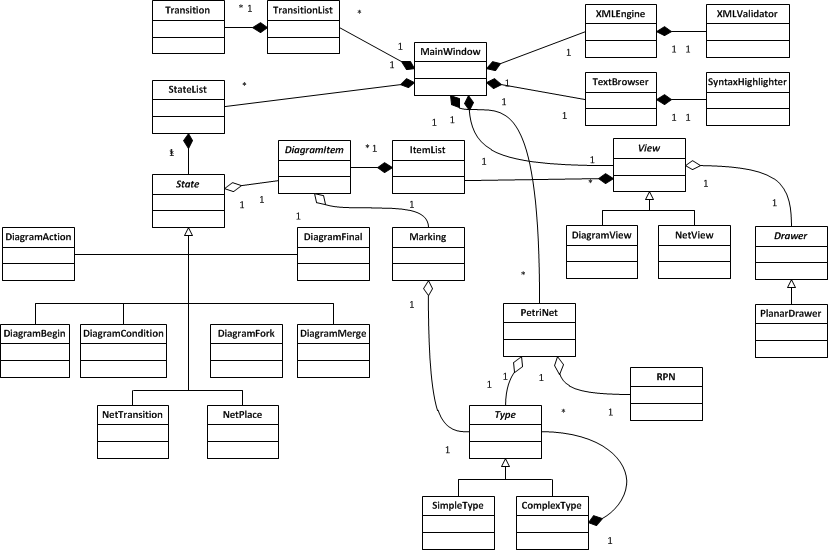
\includegraphics[scale=1]{include/ClassDiagram.png}
%	\end{center}
%	\caption{Диаграмма классов системы}
%	\label{fig:fig1}
%\end{figure}

\section{Алгоритм работы системы}

\subsection{Построение списка переменных}

Для преобразования в раскрашенную сеть Петри необходимо иметь информацию о переменных, используемых диаграммой. Переменные могут фигурировать в диаграмме в блоках действий или как спусковые функции переходов. Для разобра переменных будем использовать алгоритм поиска в глубину. Структура данных для описания типов приведена на рисунке \ref{fig:fig2}.

\begin{figure}
	\begin{center}
		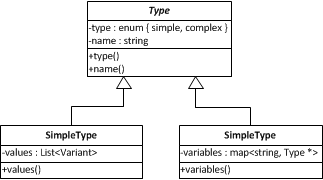
\includegraphics[scale=1]{include/Type.png}
	\end{center}
	\caption{Структура классов описание типов переменных}
	\label{fig:fig2}
\end{figure}

Все переменные можно разделить условно на два типа: простые и составные (структурные). Для простых переменных используется список сериализованных данных \textit{list<variant>}. Структурный тип имеет именнованный список переменных \textit{map<string, type *>}.	

\subsection{Преобразование в простую сеть Петри}

Условимся, что элементы преобразуются позиции и переходы. Позиции соединены с переходами, но они не имеют входных дуг, а переходы выходных. Исключения составляют начальное и конечное состояние. Так как начальное состояние имеет только одну выходную дугу, мы можем его вообще не учитывать, а выходной переход преобразуется только в соотвествующую позицию. Так как ограничения переходов могут накладываться только на блок условного перехода, при преобразовании условие преобразуется в спусковую функцию внутренней дуги между позицией и переходом.
Алгоритм преобразования состоит из двух частей:
\begin{itemize}
\item преобразование каждого элемента диаграммы в сооствествующий набор позиций и переходов сети;
\item связывание преобразовыванных элементов друг с другом.
\end{itemize}

Позиции и переходы являются наследниками абстрактного класса \textit{State}, а значит для их идентефикации используется поле \textit{id}. Для каждой позиции идентефикатор формируется как \textit{id} преобразоываемого элемента, метка \textit{place} и порядковый номер, если позиций больше одной. Аналогично для переходов. Из-за этого нарушается четкая взаимосвязь между состояниями и переходами сети, т.е. после первого этапа преобразования нельзя четко сказать какая дуга из  перехода в позицию будет соотвествовать дуге в исходном описании. Необходимо реализовать связь элементов сети, производя поиск незанятых позиций и переходов.
\begin{lstlisting}[style=pseudocode,caption={Алгоритм преобразования в простую сеть Петри}]
List<State *> queue
State * state = states.find(begin_state)
queue.append(state)

while !queue.empty():
	State * state = queue.takeFirst()
	if !netStates->find(state->id()):
		convertState(state)

	foreach transition in state.outgoing:
		if !netStates->find(target->id()):
			queue.append(target)
			convertState(target)

		if state->type() != begin_state:
			State * transition, * place;
			List<State *> transitions = netStates->find(state->id() + "transition")
			if state->type() = condition_state:
				transition = findFreeTransition(transitions)
			else
				transition = transitions.first()

			List<State *> places = netStates->find(target->id() +  "place");
			if target->type() == merge_state:
				place = findFreePlace(places)
			else
				place = places.first()

			Transition * tr = new Transition(state->id() + "-" + target->id())
\end{lstlisting}

\subsection{Формирование множества активных переходов}

В процессе моделирования на каждом шаге возникает задача поиска множества активных переходов. Для решения этой задачи можно последовать двумя путями:

\begin{itemize}
\item поиск всех переходов и выделение списка активных переходов;
\item поиск всех позиций, содержащих фишки, и на основании этого построение списка возможных переходов.
\end{itemize}

Так как каждая позиция может иметь несколько исходящих переходов, а каждый переход может иметь несколько входных позиций, задача определения множества активных переходов в общем случае сводится к полному перебору. С учетом специфики преобразования диаграммы, получаем, что из одной позиции может быть несколько переходов только в случае условного перехода и все исходящие переходы для этой позиции имеют лишь одну входящую дугу. Переход может иметь несколько входных позиций только в случае слияния, а значит все позиции имеют лишь одну исходящую дугу. Для всех остальных случаев каждый переход имеет лишь одну входную дугу, а каждая позиция лишь одну исходящую.

Основываясь на этом, сформулируем алгоритм формирования множества активных переходов:
\begin{lstlisting}[style=pseudocode,caption={Алгоритм формирования множества активных переходов}]
List<Place *> list, places = states->find(place)
MultiMap<Place *, Transition *> activeTransitions
foreach place in places:
	if place->marking > 0:
		list.append(place)
		
foreach transition in place->outgoing:
	bool flag = true
	foreach place in transition->incoming:
		if place->marking = 0:
			flag = false
	if flag:
		activeTransitions.insert(place, transition)
\end{lstlisting}

\section{Анализ работоспособности программного комплекса}

\label{cha:implementation}
